% This template is provided for all the participants of the seminar ``Spatio-temporal Logics and Reasoning''
%%%%%%%%%%%%%%%%%%%%%
% Author information:
%%%%%%%%%%%%%%%%%%%%%
% Jannik Strötgen
% Institute of Computer Science
% Database Systems Research Group
% INF 348
% 69120 Heidelberg
% stroetgen@uni-hd.de
%%%%%%%
% Date: October 5, 2010
%%%%%%%

\documentclass[
	 11pt,         % font size
	 a4paper,      % paper format
	 oneside,
	 ]{article}

%%%%%%%%%%%%%%%%%%%%%%%%%%%%%%%%%%%%%%%%%%%%%%%%%%%%%%%%%%%%

% PACKAGES:

% Use German :
\usepackage[USenglish]{babel}
% Input encoding
\usepackage[utf8]{inputenc}
% Font encoding
\usepackage[T1]{fontenc}
% Einbinden von URLs:
\usepackage{url}
% Hyperref
\usepackage[bookmarks=true,colorlinks,pdfpagelabels,pdfstartview = FitH,bookmarksopen = true,bookmarksnumbered = true,linkcolor = black,plainpages = false,hypertexnames = false,citecolor = black,urlcolor=black]{hyperref}
%\usepackage{hyperref}
% Include Graphic-files:
\usepackage{graphicx}
% Include PDF links
%\usepackage[pdftex, bookmarks=true]{hyperref}
% Fuer Textsatz
\usepackage{setspace}
% For bibliography style
\usepackage[numbers]{natbib}
% for Latex symbols
\usepackage{ marvosym }
% tables
\usepackage{ tabularx }
% quates
% \usepackage[babel,german=quotes]{csquotes}
% colors
\usepackage[usenames, dvipsnames]{xcolor}
% subscript
% \usepackage{fixltx2e}
% verzeichnisse zu toc hinzufügen
\usepackage{tocbibind}
% index
\usepackage{makeidx}
\usepackage{showidx} %DEBUG: remove
% placement H for exactly here!
\usepackage{float}
% strikeout text
\usepackage[normalem]{ulem}
% tightly packed lists
\usepackage{mdwlist}
% long tables
\usepackage{longtable}
% better ruler support for tables
\usepackage{booktabs}
% source code highliting
\usepackage{minted}
% background color for listings
\definecolor{bg}{rgb}{0.95,0.95,0.95}
% neat quotes everywhere
\usepackage{epigraph}
\setlength\epigraphwidth{12cm}
\setlength\epigraphrule{0pt}
% for a glossary
\usepackage[toc,shortcuts]{glossaries}
\makeglossaries

\newglossaryentry{X3D}{
  name=X3D,
  description={An XML based scene description language and the successor of \gls{VRML}}
}
\newglossaryentry{Roundtrip3D}{
  name=Roundtrip3D,
  description={Aim to extend SSIML, a MDD approach for 3D development to full round-trip engineering. \cite{roundtrip3dwebsite}}
}

\newacronym{GPU}{GPU}{Graphical Processing Unit}
\newacronym{SVG}{SVG}{Scalable Vector Graphics}
\newacronym{R3D}{R3D}{Roundtrip3D}
\newacronym{SSIML}{SSIML}{Scene Structure and Integration Modelling Language}

\newglossaryentry{SceGraToo}{
  name=SceGraToo,
  description={\textbf{Sce}ne \textbf{Gra}ph Composition \textbf{Too}l}
}
\newglossaryentry{OpenGL}{
  name=OpenGL,
  description={Open Graphics Library. An environment for developing portable, interactive 2D and 3D graphics applications. \cite{opengl}}
}
\newglossaryentry{git}{
  name=git,
  description={A free and open source distributed version control system designed to handle everything from small to very large projects with speed and efficiency. \cite{git}}
}
\newglossaryentry{WebGL}{
  name=WebGL,
  description={A cross-platform, royalty-free web standard for a low-level 3D graphics API based on OpenGL ES 2.0. \cite{webgl}}
}
\newacronym{3D}{3D}{3 Dimensial}
\newacronym{DAG}{DAG}{Directed Acyclic Graph}
\newacronym{XML}{XML}{Extensible Markup Language}
\newacronym{VRML}{VRML}{Virtual Reality Modeling Language}
\newacronym{HTML}{HTML}{Hypertext Transfer Protocol}
\newacronym{JSON}{JSON}{JavaScript Object Notation}
\newacronym{ID}{ID}{Identifier}
\newacronym{DOM}{DOM}{Document Object Model}

\newcommand{\acr}[1]{\glsunset{#1}\acs{#1} (\acl{#1})}
% caption* for unnumbered captions
\usepackage{caption}
% put all figures at the end
\usepackage[nomarkers,figuresonly]{endfloat}
\renewcommand{\efloatseparator}{\mbox{}}
% fancy headers
\usepackage{fancyhdr}

%%%%%%%%%%%%%%%%%%%%%%%%%%%%%%%%%%%%%%%%%%%
% Titel, Autor, Seminar, Semester, Dozent %
%%%%%%%%%%%%%%%%%%%%%%%%%%%%%%%%%%%%%%%%%%%
\newcommand{\mytitle}{Web-based 3D-scene composition for further server-sided processing in the Roundtrip3D project}
\newcommand{\mytitleShort}{SceGraToo}
\newcommand{\myauthor}{Danny Arnold}
\newcommand{\myseminar}{Web-basierte Komposition von 3D-Szenen für deren}
\newcommand{\mydozent}{Prof. Jung}
\newcommand{\mydozentTwo}{Matthias Lenk}
\newcommand{\myseminarTwo}{serverseitige Weiterverarbeitung im Roundtrip3D Projekt}
\newcommand{\mysemester}{Summer Semester 2015}

% OTHER SETTINGS:
% \setlength{\parindent}{0in}
\renewcommand{\arraystretch}{1.5}

% add listoflistings to the toc
\renewcommand{\listoflistings}{
  \cleardoublepage
  \addcontentsline{toc}{section}{\listoflistingscaption}
  \listof{listing}{\listoflistingscaption}
}

\newcommand{\emptypage}[0]{
	% Empty Page
	\clearpage
	\thispagestyle{empty}
	\mbox{}
	\newpage
}

\newcommand{\headingspage}[0]{
	% Empty Page
	\clearpage
	\thispagestyle{headings}
	\mbox{}
	\newpage
}

% Pagestyle:
\pagestyle{fancy}
% \markright{\myauthor: \section}

% start indexing
\makeindex

\begin{document}

%%%%%%%%%%%%%%%%%%%%%%%%%%%%%%%%%%%%% <TITLE> %%%%%%%%%%%%%%%%%%%%%%%%%%%%%%%%%%%%%
\pagenumbering{roman}
\begin{titlepage}
% Angaben zum Seminar
\noindent
\begin{tabular}[l]{l}
TU Bergakademie Freiberg\\
Faculty for Mathematics and Computer Science\\
\mysemester\\
\end{tabular}\\
\begin{tabular}[l]{ll}
German Title: & \myseminar\\
\phantom{German Title: } & \myseminarTwo\\
Supervisor: & \mydozent\\
\phantom{Supervisor: } & \mydozentTwo\\
\end{tabular}

\vspace{4cm}
\begin{center}
\textbf{\large Bachelor Thesis} % Proseminararbeit,Studienarbeit, Interdisziplinaeres Projekt
\vspace{0.5\baselineskip}

% Titel wird ausgegeben (siehe oben)
{\huge
\mytitle
}
\end{center}

\vfill
% Persönliche Angaben
\begin{tabular}[l]{ll}
Name:           & \myauthor\\
Matriculation Number: & 52315\\
Major:    & Applied Computer Science\\
Email: & danny.arnold@student.tu-freiberg.de\\
Date: & \today \\
\end{tabular}

\end{titlepage}
\newpage
%%%%%%%%%%%%%%%%%%%%%%%%%%%%%%%%%%%%% </TITLE> %%%%%%%%%%%%%%%%%%%%%%%%%%%%%%%%%%%%

\emptypage

% Zeilenabstand
\onehalfspacing


%%%%%%%%%%%%%%%%%%%%%%%%%%%%% <Antiplagiatserklärung> %%%%%%%%%%%%%%%%%%%%%%%%%%%%%
\thispagestyle{empty}
\vspace*{100pt}
\section*{Eidesstattliche Erklärung}
Ich, \textbf{\myauthor}, versichere, dass ich diese Arbeit selbstständig verfasst und keine anderen Hilfsmittel als
die angegebenen benutzt habe. Die Stellen der Arbeit, die anderen Werken dem Wortlaut oder
dem Sinn nach entnommen sind, habe ich in jedem einzelnen Fall unter Angabe der Quelle
als Entlehnung kenntlich gemacht. Diese Versicherung bezieht sich auch auf die bildlichen
Darstellungen.
\vspace*{50pt}

Freiberg, \today \hspace{2cm} \underline{\phantom{Platz für die Unterschrift}}
\clearpage
%%%%%%%%%%%%%%%%%%%%%%%%%%%%% </Antiplagiatserklärung> %%%%%%%%%%%%%%%%%%%%%%%%%%%%%

%%%%%%%%%%%%%%%%%%%%%%%%%%%%%% <Danksagung> %%%%%%%%%%%%%%%%%%%%%%%%%%%%%%%%%%%%%%%%
% \emptypage
% \thispagestyle{empty}
% \section*{Acknowledgment} % (fold)
% \label{sec:danksagung}
%
% % Danken möchte ich allen voran \mydozent \index{Froitzheim} und \mydozentTwo \index{Jasper} für dieses Seminar und all ihre Hilfe. Des Weiteren möchte ich mich bei \citeauthor{SeminarTemplate} für sein sehr gutes Latex-Template \cite{SeminarTemplate} bedanken, welches dieser Arbeit zu Grunde liegt, aber in vielen Bereichen angepasst wurde. Eine weitere sehr große Hilfe war das WikiBook \LaTeX~\cite{WikiLatex}, auch vielen Dank an alle Autoren dieses WikiBooks. \\
%
% % Mein Dank geht auch an die fleißigen Korrekturleser Friederike Klos \index{Klos, Friederike} und Felix Kästner \index{Kästner, Felix}.
%
% % Thanks!
%
% \begin{figure}[htbp]
% 	\includegraphics[width=\textwidth]{../assets/my-little-pony-mlp-other-261396.jpeg}
% \end{figure}

% section danksagung (end)

%%%%%%%%%%%%%%%%%%%%%%%%%%%%%% <Inhaltsverzeichnis> %%%%%%%%%%%%%%%%%%%%%%%%%%%%%%%%
\emptypage
% Table of contents
\setcounter{tocdepth}{5}
\tableofcontents
\clearpage
%%%%%%%%%%%%%%%%%%%%%%%%%%%%%% </Inhaltsverzeichnis> %%%%%%%%%%%%%%%%%%%%%%%%%%%%%%%

%%%%%%%%%%%%%%%%%%%%%%%%%%%%%% <Hauptteil der Arbeit> %%%%%%%%%%%%%%%%%%%%%%%%%%%%%%
\emptypage
\pagenumbering{arabic}

% !TEX root = seminararbeit.tex

\section{Introduction}
\label{sec:Prelude}

The goal of the thesis is to create a \gls{3D} editor, using web technologies,
which enables its users to postprocess \gls{X3D} scenes. These scenes are the
product of a tool that was implemented as part of the DFG research
project \gls{Roundtrip3D} \cite{Jung:2015:SDA:2802768.2802837}.
% The scene are automatically derived from software models \ldots{}
\subsection{Motivation}\label{motivation}

As part of the Roundtrip3D project, a round-trip framework (hereafter
referred to as \emph{R3D}) was developed. This framework also includes a
graphical editor for SSIML models, to describe \gls{3D} applications. Then
\gls{R3D} can be used to generate boilerplate code for multiple programming
languages, such as JavaScript, Java or C++, and an \gls{X3D} file describing
the scene. The \gls{X3D} file may contain references to other \gls{X3D} files
containing the actual \gls{3D} data (e.g.~a car and its corresponding tires),
hereafter called \emph{inlines}. These files are created by exporting
objects from a \gls{3D} computer graphics software (e.g.~Blender,
Maya or 3DS Max).\\
The problem that arises is that each object is usually in the center of
its own coordinate system. So they need to be translated, rotated and
maybe even scaled, to result in the desired scene (e.g.~a car where the tires
are in the places they belong to and not in the center of the chassis).
The structure is mostly generated. Attribute values of respective nodes,
such as transformation nodes, need to be adjusted in order to compose the
overall \gls{3D} scene.

% \includegraphics{Picture of a car with the tires in the center}\\
% \includegraphics{Picture of a car with the tires where they belong to}

This can be achieved by adjusting \emph{translate}, \emph{rotate} and
\emph{scale} properties to arrange \gls{3D} objects. To exacerbate this problem
further, the orientation the \gls{3D} artists chose for its object may be unknown, if
% TODO: so what now? convention or no convention?
their is no convention for \gls{3D} modeling. \sout{Usually their is a convention
about origin of coord system, scaling and orientation} (no there isn't, still
not sure what to put here). However, we cannot assume that these conventions are
always met. The main problem is, that \gls{3D} transformations, such as translation,
orientation and scale of single \gls{3D} geometries, need to be adjusted. So far,
there is no graphical tool that meets both of these requirements:

\begin{itemize*}
  \item User friendly and straight forward composition functionalities for \gls{X3D} scenes and
  \item preservation of (generated) information, such as node names or comments (necessary to merge the changed files back into the source model).
\end{itemize*}

\begin{figure}
  \begin{minipage}{.5\textwidth}
    \includegraphics[width=0.9\textwidth]{../assets/wheel1.png}
  	\caption{One possible orientation.}
  	\label{fig:wheel1}
  \end{minipage}
  \begin{minipage}{.5\textwidth}
  	\includegraphics[width=0.9\textwidth]{../assets/wheel2.png}
  	\caption{Another possible orientation.}
  	\label{fig:wheel2}
  \end{minipage}\\
  \begin{minipage}{.5\textwidth}
  	\includegraphics[width=0.9\textwidth]{../assets/wheel3.png}
  	\caption{Yet another possible orientation.}
  	\label{fig:wheel3}
  \end{minipage}
  \begin{minipage}{.5\textwidth}
  	\includegraphics[width=0.9\textwidth]{../assets/wheel4.png}
  	\caption{An improbable orientation, unless the \gls{3D} artist was very confused.}
  	\label{fig:wheel4}
  \end{minipage}
  \caption*{Four possible orientations the \gls{3D} model of a wheel could have.}
\end{figure}

Figures \ref{fig:wheel1} - \ref{fig:wheel4} demonstrate multiple orientatins a \gls{3D} model of a wheel can have. \ref{fig:wheel1} to \ref{fig:wheel3} are common
orientations, since it is disputable which of these could be considered be the
norm. But if one depends on art from 3rd parties, the orientation and position
could be completely arbitrary like in figure \ref{fig:wheel4}

These properties could be added and adjusted via any text editor by opening the
generated \gls{X3D} file, but the resulting workflow is not user-friendly. The
following list explains the workflow using just a text editor.

\begin{enumerate*}
  \item Model the \gls{3D} application, including \gls{3D} the scene structure.
  \item Generate the \gls{3D} scene and the application code.
  \item Run the application and evaluate the scene and think about what objects need to go where and whether they need to be scaled.
  \item Type random translation, rotation and scale values into the transform nodes.
  \item Run the application again and evaluate whether the transformations are correct (since one does not know anything about the orientation of the object).
  \item Go back to 4. until all objects are placed correctly.
\end{enumerate*}

Tools like Maya or Blender could also be used for this, but their import
and export filter discard important metadata that is necessary for the
round-trip transformation. This is what \gls{Roundtrip3D} is meant to be. \gls{Roundtrip3D} addresses both of these issues. It allows for loading the root \gls{X3D} file and changing all transformations, containing the inline nodes,
using mouse interactions. For fine grained control \gls{Roundtrip3D} also
contains a tree view that allows the user to input exact attributes for
translations, rotations and scale.

\subsection{Scope}\label{scope}

This thesis addresses two issues:

\begin{enumerate*}
  \item Allowing for composing generated \gls{X3D} scenes (with focus on usability). E.g., besides a \gls{3D} view, a tree view for fine grained editing should not only visualize the \gls{3D} scene's structure, but also allow for entering concrete coordinate values.
  \item During the editing process, the preservation of all information/metadata must be guaranteed.
\end{enumerate*}


% !TEX root = seminararbeit.tex

\section{Basics and Related Work}
\label{basics-and-related-work}

\subsection{Scene-Graph}\label{scene-graph}

Scene-graphs can be used to group and organize 3D objects, their
properties and concerning transformations. A directed acyclic graph
(DAG) can be used to represent a scene-graph. It starts with a root node
that is associated with one or more children. Each child can be an
object or a group, again containing more children. A group can contain
associated transformation information, like \emph{translation},
\emph{rotation} or \emph{scaling}. This structure has certain advantages
compared to applying all transformations to the raw meshes and sending
everything to the \gls{GPU}. \cite{realityprime}

\gls{SSIML} \cite{Lenk:2012:MID:2338714.2338742} scene-graphs differ from the above definition:
there are three types of nodes:
\begin{itemize*}
  \item transform
  \item geometry
  \item group
\end{itemize*}

\subsubsection{Culling}\label{culling}

Before using structures like scene-graphs, all polygon would be sent to
the \gls{GPU} and the \gls{GPU} would need to test what polygons are actually in the
view and thus need to be rendered. The problem with that approach was
that this information was only known after doing a lot of calculations
for every polygon already.\\
With a scene-graph it's possible to start from the root and traverse the
graph, testing the bounding box of each group and only sending it to the
\gls{GPU} it it's completely visible. If it ain't, the whole sub-tree isn't
sent to the \gls{GPU}. If it's partially visible the same process is applied
to the sub-tree.\\
By using a structure that retains more information about what it
represents it's possible to let the CPU do more of the heavy
lifting and unburden the \gls{GPU}.

\begin{quote}
  Rather than do the heavy work at the OpenGL and polygon level,
  scene-graph architects realized they could better perform culling at
  higher level abstractions for greater efficiency. If we can remove the
  invisible objects first, then we make the hardware do less work and
  generally improve performance and the all-important frame-rate. \cite{realityprime}
\end{quote}

\subsubsection{Transformations}\label{transformations}

Another advantage is the way transformations work. Instead of applying
them to the meshes directly, and keeping track of what meshes belong to
the same object (like the chassis and the tires and the windows of a
car), they can simply be nested under the same transformation group. The
transformation thus applies to all objects associated with that group.

\subsubsection{Reuse}\label{reuse}

With the ability to address nodes it's possible to reuse their
information. If you have a car, it would be enough to have only one node
containing the geometry for a tire, all other tires are merely addressing
the tire with the geometry information (see listing \ref{list:defuse}).
That way the memory footprint of an application can be reduced.

\begin{figure}
  \begin{minted}{html}
<Group>
  <Transform>
    <Shape def="chassis">
        <Appearance>
            <Material></Material>
        </Appearance>
        <Box></Box>
    </Shape>
  </Transform>
  <Transform>
    <Shape def="tire">
        <Appearance>
             <Material></Material>
        </Appearance>
        <Torus></Torus>
    </Shape>
  </Transform>
  <Transform>
    <Shape use="tire"/>
  </Transform>
  <Transform>
    <Shape use="tire"/>
  </Transform>
  <Transform>
    <Shape use="tire"/>
  </Transform>
</Group>
  \end{minted}
  \caption{example x3d group showing the use of \texttt{def} and \texttt{use}}
  \label{list:defuse}
\end{figure}


\subsection{X3D}
\label{x3d}

X3D is the XML representation of VRML which was designed as
a universal interactive 3D exchange format, much like html is for
written documents or \gls{SVG} for vector graphics. Due to its XML structure
it can be integrated in html documents, thus the Frauenhofer Institute
pursued to implement a runtime that could interpret and visualize X3D in
the browser, by using a WebGL context. It's called
\href{http://www.x3dom.org/}{x3dom} and it's extensively used by
SceGraToo, the tool that arose from this thesis.

\subsubsection{x3dom}
\label{par:x3dom}

As said in the previous chapter x3dom was developed by the Frauenhofer
Institute to realize the vision that started VRML in the first place:
\emph{mark up interactive 3D content for the web}. On the web there are
to entirely different approaches to describe the same thing:
\begin{itemize*}
  \item imperative
  \item declarative
\end{itemize*}

The matrix in table \ref{tab:feature_matrix} classifies x3dom together with other common web
technologies \cite{x3dom}:

\begin{table}[H]
  \begin{longtable}[c]{@{}lll@{}}
  \toprule
  & 2D & 3D\tabularnewline
  \midrule
  \endhead
  Declarative & \gls{SVG} \cite{svg} & x3dom \cite{x3dom} \tabularnewline
  Imperative  & Canvas \cite{canvas} & WebGL \cite{webgl} \tabularnewline
  \bottomrule
  \end{longtable}
  \caption{\cite{x3dom}}
  \label{tab:feature_matrix}
\end{table}

As can be seen in table \ref{tab:feature_matrix} x3dom complements the already existing technologies
perfectly.

\subsection{SSIML}
\label{ssiml}

Heterogeneous developer groups, groups that are comprised of people from
different backgrounds (programmers, 3D designers) have hard time working
together. \cite{Glinz:2015:SUS:2802768.2802838}

SSIML is a graphical approach to unify the scene-graph model and the the
application model, thus making the communication between the different
parties easier.

It also serves as a code generation template.

\begin{figure}[htbp]
  \centering
  \includegraphics[width=12cm]{../assets/SSIML.png}
	\caption{A SSIML Diagram \cite{roundtrip3dwebsite}}
	\label{fig:ssimldiagram}
\end{figure}

\subsection{Roundtrip 3D}\label{roundtrip-3d}

As stated above, when developing 3D applications, many different
developers are involved, i.e.~3D designers, programmers and, ideally,
also software designers (see figure \ref{fig:ssimldiagram})

% TODO: convert to pdf
% 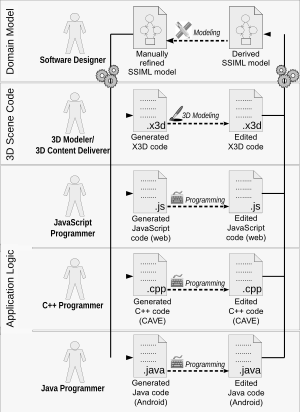
\includegraphics{../assets/csrd2014.svg}\\
% Roundtrip3D proposed process
% \href{http://dx.doi.org/10.1007/s00450-014-0258-8}{JLV15}

Roundtrip3D was research project that, amongst others, resulted in a
graphical editor for \hyperref[ssiml]{SSIML} models. It offers an
approach for merging a developer's changes back into the main model.
After all working copies are merged back into the main model (dropping
unwanted or conflicting changes), all working copies are regenerated and
delivered to the individual developers. After each roundtrip every
developer has a copy of the project that is consistent with everyone
else's.

\subsection{Related Work}
\label{related-work}

\subsubsection{Collaborative Work}
\label{collaborative-work}

\subsubsection{\texorpdfstring{\href{http://3d.meteor.com/}{3D
Meteor}}{3D Meteor}}\label{d-meteor0}

\begin{figure}[htbp]
  \centering
  \includegraphics[width=12cm]{../assets/3dmeteor.png}
  \caption{3D Meteor}
	\label{fig:3dmeteor}
\end{figure}

This simple 3D editor allows the user to add and remove colored blocks
to a scene. The synchronization is leveraging meteor's database
collection subscription features. Meteor apps are comprised of a client
side and a server side. The client can subscribe to database collections
and get's automatically notified of changes to that collection by the
server. The only thing that actually is synchronized is an array of
\emph{boxes}. A box is an object with an x, y and z property describing
its position.

\subsubsection{Blender Plugin}
\label{blender-plugin}

I don't do anything about collaborative working anymore. So yeah.

As part of an asset management system the Université du Québec à
Montréal implemented a plugin for blender for collaborative working. An
artist can record changes to to wiremeshes and store them on a server.
Another artist can download these changes and apply them to his working
copy. The diffs are a simple list of vertices and their movement in the
x, y and z space. \cite{LCR07}

\begin{verbatim}
95 [0.0000, 0.0000, 0.0000]
295 [0.0027, 0.0013, 0.0000]
309 [0.2123, 0.1001, 0.0000]
311 [0.3029, 0.1429, 0.0000]
\end{verbatim}

These are saved on the server and another user working on the same
object can apply them to his working copy. They can actually be applied
to any object that has the same number of vertices. That's also a
shortcoming. Adding or removing vertices cannot be handled by the
plugin. It is also not in real time, so it is more comparable to version
control system like git, just for 3d models.

\subsubsection{Tilt Brush}
\label{tilt-brush20}

Tilt Brush was lauded for it's 3d interface.

\subsubsection{Gizmos}\label{gizmos}

Gizmos, also called manipulators, are handles or bounding boxes with
handles that manipulate it's containgin object in a predefined way when
dragged. \cite{wikigizmo}

In X3D gizmos can be realized with on of X3DDragSensorNode's \cite{x3ddragsensornode} decedents.

\begin{description*}
\item[SphereSensor]
  SphereSensor converts pointing device motion into a spherical rotation around the origin of the local coordinate system. \cite{spheresensor}
\item[CylinderSensor]
  The CylinderSensor node converts pointer motion (for example, from a mouse) into rotation values, using an invisible cylinder of infinite height, aligned with local Y-axis. \cite{cylindersensor}
\item[PlaneSensor]
  PlaneSensor converts pointing device motion into 2D translation, parallel to the local Z=0 plane. Hint: You can constrain translation output to one axis by setting the respective minPosition and maxPosition members to equal values for that axis.
  \cite{planesensor}
\end{description*}

The sensors track drag events on their siblings. In the example in figure \ref{fig:x3dgizmo}
(which is taken directly from the x3dom website) the PlaneSensor tracks
drag events on the cones and the cylinder that make up the cyan handle.

Every time it detects a drag event it converts it into a 2D
transformation and raises an \emph{onOutPutChange} event. The callback
\texttt{processTranslationGizmoEvent} is registered as an event handler.
In this function the position of the handle is adjusted to make it
follow the drag movement, also the position of the teapot is adjust.

Having the the handles being 3d objects within the scene, that look
touchable and intractable, make it easier for users find their way
around the application. Instead of haven to learn keyboard shortcuts the
user simply uses their intuition about how she would interact with
objects in the real world.

\begin{minted}[breaklines,bgcolor=bg]{html}
<group>
  <planeSensor autoOffset='true' axisRotation='1 0 0 -1.57' minPosition='-6 0' maxPosition='6 0' onoutputchange='processTranslationGizmoEvent(event)'>
  </planeSensor>

  <transform id='translationHandleTransform'>
    <transform translation='0 -5.5 8' rotation='0 1 0 1.57'>
      <transform translation='0 0 1.5' rotation='1 0 0 1.57'>
        <shape DEF='CONE_CAP'>
          <appearance DEF='CYAN_MAT'><material diffuseColor='0 1 1'></material></appearance>
          <cone height='1'></cone>
        </shape>
      </transform>
      <transform rotation='1 0 0 -1.57'>
        <shape>
          <appearance USE='CYAN_MAT'></appearance>
          <cylinder></cylinder>
        </shape>
      </transform>
      <transform translation='0 0 -1.5' rotation='1 0 0 -1.57'>
        <shape USE='CONE_CAP'></shape>
      </transform>
    </transform>
  </transform>
</group>
\end{minted}

\begin{figure}[htbp]
  \begin{minipage}{.5\textwidth}
    \centering
    \includegraphics[width=0.9\textwidth]{../assets/Manual-Manipulators-Translate.jpg}
  	\caption{translation gizmo \cite{blenderwiki}}
  \end{minipage}
  \begin{minipage}{.5\textwidth}
    \centering
    \includegraphics[width=0.9\textwidth]{../assets/Manual-Manipulators-Translate.jpg}\\
  	\caption{rotation gizmo \cite{blenderwiki}}
  \end{minipage}\\
  \begin{minipage}{.5\textwidth}
    \centering
    \includegraphics[width=0.9\textwidth]{../assets/Manual-Manipulators-Scale.jpg}
  	\caption{scale gizmo \cite{blenderwiki}}
  \end{minipage}
  \begin{minipage}{.5\textwidth}
    \centering
    \includegraphics[width=0.9\textwidth]{../assets/Manual-Manipulators-Combo.jpg}
  	\caption{all gizmos together \cite{blenderwiki}}
  \end{minipage}
\end{figure}
\begin{figure}[]
  \centering
  \includegraphics[width=12cm]{../assets/threejs-editor.png}
	\caption{ Shows translate gizmos along the x, y and z axis als well as gizmos that translate the cube along the xy, xz, yz and frustum plane. \cite{threejseditor} }
\end{figure}
\begin{figure}[]
  \centering
  \includegraphics[width=12cm]{../assets/x3dom-gizmo-example.png}
	\caption{ Shows an official x3dom tutorial for using sensors to create gizmos. \cite{x3dgizmo} }
	\label{fig:x3dgizmo}
\end{figure}

\clearpage

\subsubsection{Component Editor}
\label{component-editor30}

On the 12th of June 2015 the x3dom maintainers released their Component Editor. \cite{componenteditor}
It was released after the my work on SceGraToo started.
Its development took about a year and three people working part-time on it. \cite{componenteditoreffort}
Although it does offer all the wanted scene composition features, it lacks the ability to:

\begin{itemize*}
  \item load an existing x3d file
  \item save the scene as an x3d file
  \item upload x3d files that can be included as inlines
\end{itemize*}

Scenes can only be loaded and saved as a json representation (see listing~\ref{componenteditorjson}).
Conversion between the formats may be possible, but meta information like IDs in comments would be lost.

\begin{listing}
  \begin{minted}[breaklines,bgcolor=bg]{json}
{
  "0": {
    "type": "Box",
    "transform": "1.000000, 0.000000, 0.000000, 0.000000, \n0.000000, 1.000000, 0.000000, 0.000000, \n0.000000, 0.000000, 1.000000, 0.000000, \n0.000000, 0.000000, 0.000000, 1.000000",
    "referencePoints": ["p1", "p2", "p3", "p4", "p5", "p6"],
    "parameters": {
      "Size": [1, 1, 1],
      "Positive Element": "true"
    }
  }
}
  \end{minted}
  \caption{}
  \label{componenteditorjson}
\end{listing}

\subsubsection{Real-Time Collaborative Scientific WebGL Visualization with Web Sockets}
\label{rtcswvwws}

Using web sockets instead of AJAX is an interesting approach. \cite{Marion:2012:RCS:2338714.2338721} Especially
the cut down on latency. It is over all very similar to the approach I
was thinking about. Except that they propagate only some information,
like the camera position and view angle. In SceGraToo's case the whole
scene needs to be synchronized. So to have specttors like they have we
either have to send the whoe model to the server after eacht change or
use some kind of tree diff algorithm. They visualize a specific dataset
in a threejs's specific JSON format \cite{threejs-format}. We only need to visualize X3D
data, so there is no reason to use some generic Visualization tool kit,
x3dom does a pretty good job doint this. on the other hand we not only
have to visualize the data, but also manipulate it and this is way
easiear in a descriptive scene graph instead of manimpulatiing webgl
scenes or data formats like vtk.

\subsubsection{ParaViewWeb pvweb}
\label{paraviewweb-pvweb}

Simple to use out of the box, but needs a paraview server instance and
paraview does not support x3d as an input format. So using this is sadly
not possible unless an import filter is written. The visualization is
mainly meant to explore data sets. There is no easy way to manipulate
the input data. This can only happen by extending the visualization
pipeline via python scripts on the server.


% !TEX root = seminararbeit.tex

\section{Concept}
\label{concept}

% TODO: skizze wie dom rendering funktioniert oder auch nicht, da es ziemlich uninteressant ist

In the following sections the initial design concept of \gls{SceGraToo} is illustrated.

\subsection{Server}
\label{server}

% TODO: put text here

\subsubsection{Node.js}
\begin{quote}
  ``Node.js is a platform built on Chrome's JavaScript runtime for easily building fast, scalable network applications. Node.js uses an event-driven, non-blocking I/O model that makes it lightweight and efficient, perfect for data-intensive real-time applications that run across distributed devices.'' \cite{nodejs}
\end{quote}

Node is used because it is inherently easy writing small servers with it, and
SceGraToo's server is not going to be complex. \footnote{Complex servers can be
written in Node.js as well. It is just not encouraged, since most people tend to
refactor their infrastructure into micro services.}

Listing \ref{list:nodejs} shows a server that is looking up a user from the database and returning it as \gls{JSON} to the browser.

\begin{listing}
  \begin{minted}[breaklines,bgcolor=bg,linenos=true]{javascript}
const http = require('http')
const db = require('db')

http.createServer((request, response) => {
  db.getuser(function(error, user) {
    if (error) {
      return res.status(404).send(error);
    } else {
      response.writeHead(200, {'Content-Type': 'application/json'})
      response.send(user)
    }
  })
}).listen(1337, '127.0.0.1')
  \end{minted}
  \caption{An example server in Node.js, using the http module in its standard library.}
  \label{list:nodejs}
\end{listing}

\subsubsection{Koa}
\label{par:Koa}
\begin{quote}
  ``Koa is a new web framework designed by the team behind Express, which aims to be a smaller, more expressive, and more robust foundation for web applications and APIs. Through leveraging generators Koa allows you to ditch callbacks and greatly increase error-handling. Koa does not bundle any middleware within core, and provides an elegant suite of methods that make writing servers fast and enjoyable.'' \cite{koajs}
\end{quote}

Koa is used to make writing the server, and using asynchronouse functions in request handlers simpler and clearer.
See Listing \ref{list:koajs} for the same example from Listing \ref{list:nodejs} written with koajs.
It is not only shorter, but also simplier and clearer.

\begin{listing}
  \begin{minted}[breaklines,bgcolor=bg,linenos=true]{javascript}
const db = require('db')
const koa = require('koa')
const app = koa()

app.use(function * (){
  this.body = yield db.getUser()
})

app.listen(3000)
  \end{minted}
  \caption{An example server utilizing the Koa framework.}
  \label{list:koajs}
\end{listing}

\subsection{Client}
\label{client}

\epigraph{``I conclude that there are two ways of constructing a software design:
One way is to make it so simple that there are obviously no deficiencies
and the other way is to make it so complicated that there are no obvious
deficiencies. The first method is far more difficult.''}{--- Hoare, Turing Award Lecture 1980}

The tree-view is the most important part of SceGraToo. It shows the
structure rather than the visual representation. Different
off-the-shelf solutions, like angular or JQuery plugins, were tested
against the following requirements:

\begin{enumerate*}
  \item Custom \gls{HTML} elements as part of tree nodes (e.g.~multiple checkboxes or multiple inputs),
  \item ability to observe the tree node's state changing,
  \item binding to an arbitrary model and
  \item detecting inconsistencies between the model and the view and recovering from them.
\end{enumerate*}

\textbf{Partially not met requirements:}

\begin{itemize*}
  \item Custom elements as part of tree nodes and
  \item ability to listen to changes to the tree node.
\end{itemize*}

\textbf{Requirements none of the tested tools met:}

\begin{itemize*}
  \item Binding to an arbitrary model and
  \item detecting inconsistencies between the model and the view and recovering from them.
\end{itemize*}

None of the off-the-shelf solutions could satisfy all expectations. After
evaluating a couple of solutions it was clear that the problem space was too
specific and a custom solution is required.

\subsubsection{Synchronization Process}

Of all requirements, the most complicated part is keeping the tree-view in sync
with the scene-graph, while the scene-graph is being modified and vice
versa.

\paragraph{Terminology}
\label{terminology}

\begin{description*}
  \item[scene-graph:]
    The \gls{X3D} representation of the scene as part of the \gls{DOM}, see Listing~\ref{list:x3dscene} and the screenshot in Figure \ref{fig:x3dom-dom} from the Chrome DevTools.
  \item[scene-graph-node:]
    A specific scene graph node (e.g.~\texttt{inline}, \texttt{transform} or \texttt{scene}).
  \item[tree-view-component:]
    Comprises all functionality related to parsing the scene-graph and creating the tree-view out of individual tree-view-node-components.
  \item[tree-view:]
    The \gls{HTML} representation of the tree-view-component as part of the \gls{DOM}, see Figure \ref{fig:tree-view} and Listing \ref{list:tree-view} (\gls{HTML} output
    shortened and simplified).
  \item[tree-view-node-component:]
    Comprises all functionality related to synchronizing changes from a scene-graph-node to the corresponding
    tree-view-node and vice-versa.
  \item[tree-view-node:]
    The \gls{HTML} representation of the tree-view-node-component as part of the \gls{DOM}, see Figure \ref{fig:tree-view-node-dom} and Figure \ref{fig:tree-view-node-rendered}.
\end{description*}

\begin{figure}
  \centering
  \includegraphics[width=\textwidth]{../assets/treeview.png}
  \caption{The rendered tree-view.}
  \label{fig:tree-view}
\end{figure}

\begin{figure}
  \centering
  \includegraphics[width=\textwidth]{../assets/x3dom-dom.png}
  \caption{The \gls{X3D} scene inside the \gls{DOM}.}
  \label{fig:x3dom-dom}
\end{figure}

\begin{figure}
  \centering
  \includegraphics[width=\textwidth]{../assets/treeview-dom.png}
  \caption{About half of the \gls{DOM} elements that make up a tree-view of only three tree-view-nodes: a \texttt{scene}, a \texttt{transform} and an \texttt{inline}.}
  \label{fig:treeview-dom}
\end{figure}

\begin{figure}
  \centering
  \includegraphics[width=\textwidth]{../assets/treeview-node-dom.png}
  \caption{The \gls{DOM} elements that make up a tree-view-node for an \texttt{inline}.}
  \label{fig:tree-view-node-dom}
\end{figure}

\begin{figure}
  \centering
  \includegraphics[width=.5\textwidth]{../assets/tree-view-node-rendered.png}
  \caption{The rendered tree-view-node of an \texttt{inline}.}
  \label{fig:tree-view-node-rendered}
\end{figure}

\begin{listing}
  \begin{minted}[breaklines,bgcolor=bg,linenos=true]{html}
<x3d version="3.0" profile="Interaction" width="708px" height="354px">
<!-- id=69b81d54-6e7a-4967-acca-b8c89ba90782 -->
<scene render="true" bboxcenter="0,0,0" bboxsize="-1,-1,-1" pickmode="idBuf" dopickpass="true">
<worldinfo>
</worldinfo>
<background skycolor="0.3 0.3 0.3"></background>
<viewpoint fieldofview="0.7" position="1 1 3" orientation="0.1 0.9 0.13 3.8">
</viewpoint>
<!-- id=8d3f0a8a-b6d7-4acc-922b-ea59364443fa -->
<group render="true" bboxcenter="0,0,0" bboxsize="-1,-1,-1">
  <transform render="true">
    <!-- id=8459b736-5a9d-4688-b624-e519857a92fd -->
    <inline url="projects/Red Box/src/redBox.x3d" render="true" load="true">
      <Shape render="true" isPickable="true">
        <Appearance sortType="auto" alphaClipThreshold="0.1">
          <Material diffuseColor="1 0 0" ambientIntensity="0.2" shininess="0.2"></Material>
        </Appearance>
        <Box solid="true" size="2,2,2"></Box>
      </Shape>
    </inline>
  </transform>
</group>
</scene>
</x3d>
  \end{minted}
	\caption{ \gls{X3D} example scene.}
	\label{list:x3dscene}
\end{listing}

\begin{listing}
  \begin{minted}[breaklines,bgcolor=bg,linenos=true]{html}
<div>
  <li>
    <div>
      <a> <span>SCENE</span> </a>
    </div>
    <div>
      <div>
        <div>
          <div>
            <span>render:</span>
          </div>
          <div>
            <input type="checkbox">
          </div>
        </div>
      </div>
      <ol>
        <li>
          <div>
            <a> <span>WORLDINFO</span> </a>
            <a>X</a>
          </div>
          <div>
            <div>
              <div>
                <div>
                  <span>def:</span>
                </div>
                <div>generatedWorldInfo1</div>
              </div>
            </div>
          </div>
...
      </ol>
    </div>
  </li>
</div>
  \end{minted}
  \caption{Example of a tree-view, the structure is simplified.}
  \label{list:tree-view}
\end{listing}

The aim is to keep the tree-view a consistent representation of the scene-graph.
The tree-view filters some nodes and attributes. As an example, nodes contained
in an \texttt{inline} are not shown, since  SceGraToo's task is only to compose
a scene of \texttt{inlines}, not to change anything inside the \texttt{inlines}.
Also not all attributes are shown, but only the ones the user may be interested
in (such as \texttt{DEF}, \texttt{translate} or \texttt{rotate}).

One approach is to instantiate the tree-view-component with a
scene-graph-node as root node. For all child nodes, the tree-view-component
instatiates new tree-view-node-components. These tree-view-node-components
create the corresponding tree-view-nodes, while further traversing the
scene-graph. For each scene-graph-node a corresponding tree-view-node-component
is created. If there are no child nodes left, the tree-view creation is done.
Each tree-view-node-component creates all \gls{DOM} elements necessary to represent
the corresponding scene-graph-node in the \gls{DOM}. Also each
tree-view-node-component observes its corresponding scene-graph-node for
attribute mutations and added or removed child nodes and acts accordingly.

Depending on how the scene-graph is mutated, three main cases can be differentiated:

\begin{description*}
  \item[a scene-graph-node is added]
    A new tree-view-node-component is instantiated, adding all \gls{DOM} elements making up the tree-view-node to the \gls{DOM}.
  \item[a scene-graph-node is deleted]
    The corresponding tree-view-node-component is destroyed and all \gls{DOM} elements making up that tree-view-node are removed from the \gls{DOM}.
  \item[a scene-graph-node is mutated]
    The corresponding \gls{DOM} elements that make up the  tree-view-node are altered to reflect the mutation.
\end{description*}

Tree-view-nodes can also be used to edit scene-graph nodes' properties. When an
input element, that contains the x value of a transformation, is edited, its
tree-view-node-component is notified of the change, by firing a change event, to
which the component subscribed, and applies the new value to the corresponding
scene-graph-node.

It is assumed, that the updates will always lead to consistent a state, where the
scene-graph and the tree node converge. It is also assumed, that an application
may be buggy and in that case the synchronization process has no ability to
detect if updates lead to an inconsistent state. It also has no ability to
recover from an inconsistent state, though without the ability to detect
inconsistencies this does not really matter.

In the following, the two main problems are described.

\begin{description*}
  \item[Problem 1: keeping the tree-view consistent with the scene-graph]
    The difficulty, to make sure that incremental updates are error-free,
    exacerbates even more when further functionality is
    added to the tree-view,  like checkboxes for
    specific properties or saving state in the tree-view that is not part of
    the scene-graph, e.g~the possibility to collapse parts of the tree.
  \item[Problem 2: implementation effort]
    For every new feature four things have to implemented:
    \begin{enumerate*}
      \item Code for parsing the scene-graph
      \item Code to generate the tree-view-node
      \item Code to synchronize changes to a scene-graph-node to the corresponding tree-view-node
      \item Code to synchronize changes to a tree-view-node to the corresponding scene-graph-node
    \end{enumerate*}
\end{description*}

This can be greatly simplified if only the functionality for parsing the
scene-graph, and  for creating the \gls{DOM} elements that represent the scene-graph,
is implemented and on every change the whole tree-view is recreated by doing
this again.

Problem 1 disappears completely, because the incremental updates are gone and
Problem 2 is reduced to the following two steps:

\begin{enumerate*}
  \item Code for parsing the scene-graph and generating the tree-view
  \item Code to synchronize changes to a tree-view-node to the corresponding scene-graph-node
\end{enumerate*}

Rerendering everything on every change is usually inefficient. Removing a big part
of the \gls{DOM} and replacing it would kick of a \emph{reflow}, which is the browser's
process of laying out the content. This process is blocking, meaning the user can't
scroll or otherwise interact with the application. \cite{reflow}

React is used to minimize the possibility of a reflow happening. React
calculates a lightweight representation of what the \gls{DOM} should be like and
compares that to what the \gls{DOM} is already. It calculates a set of patches and
only applies these to the \gls{DOM}.

From a developer's point of view the application is programmed like it is
completlely rerendered everytime something changes. But from the browser's point
of view only a minimal set of changes, only those that are required to transform the
\gls{DOM} into the disired state, are applied, thus greatly reducing the risk of a \emph{reflow}.

The code below (Listings \ref{oldvirtdom}, \ref{newvirtdom} and \ref{patch}) is
for explanitary purposes to describe how react works. It does not resemble
react's implementation in any way:

\begin{listing}[H]
  \begin{minted}[breaklines,bgcolor=bg,linenos=true]{html}
<ol data-reactid=".0">
  <li data-reactid=".0.0">scene
    <ol data-reactid=".0.0.0">
      <li data-reactid=".0.0.0.0">transform
        <ol data-reactid=".0.0.0.0.0">
          <li data-reactid=".0.0.0.0.0.0">inline</li>
        </ol>
      </li>
    </ol>
  </li>
</ol>
  \end{minted}
  \caption{Old Virtual DOM}
  \label{oldvirtdom}
\end{listing}

\begin{listing}[H]
  \begin{minted}[breaklines,bgcolor=bg,linenos=true]{html}
<ol data-reactid=".0">
  <li data-reactid=".0.0">scene
    <ol data-reactid=".0.0.0">
      <li data-reactid=".0.0.0.0">transform
        <ol data-reactid=".0.0.0.0.0">
          <li data-reactid=".0.0.0.0.0.0">inline</li>
        </ol>
      </li>
      <li>group</li>
    </ol>
  </li>
</ol>
  \end{minted}
  \caption{New Virtual DOM}
  \label{newvirtdom}
\end{listing}

\begin{listing}[H]
  \begin{minted}[breaklines,bgcolor=bg,linenos=true]{javascript}
var li = document.createElement('li')
li.innerText = 'group'
document.querySelector('[data-reactid=".0.0.0"]')
  .appendChild(li)
  \end{minted}
  \caption{Patch}
  \label{patch}
\end{listing}

That means, as long as the code that parses the scene-graph and generates the
lightweight representation of the tree-view is correct, the tree-view will
represent the current state of the scene-graph.

\paragraph{Data Binding}
\label{data-binding}

Another idea is to utilize templates and data binding. Frameworks (like
angular) or web components implementations (like polymer)
support templates and two way data binding. Following only
angular directives are examined, but the same should be possible with web
components.

An angular directive consists of a mostly logicless template and some
javascript containing logic for creating the directive or reacting to
events.

For each node a directive is instantiated, which creates a template
rendering the node. Also for each child it creates a new instance of
itself.

\textbf{Example:}

The rendered structure is shown in Listing \ref{list:templatedata}. The
\texttt{treenode} (Listing \ref{list:angular1}) expands into the node name and a
\texttt{nodelist} (Listing \ref{list:angular2}), that then expands into a list
of tree-nodes for each child node (Listing \ref{list:angular3}), that further
expand again (Listing \ref{list:angular4}). This recursive expanding stops when a
\texttt{treenode} is childless.

\begin{listing}[H]
  \begin{minted}[breaklines,bgcolor=bg,linenos=true]{javascript}
node: {
  name: "scene",
  children: [
    {
      name: "viewpoint"
    },
    {
      name: "worldinfo"
    }
  ]
}
  \end{minted}
  \caption{Example input data.}
  \label{list:templatedata}
\end{listing}

\begin{listing}[H]
  \begin{minted}[breaklines,bgcolor=bg,linenos=true]{html}
<treenode node="node">
</treenode>
  \end{minted}
  \caption{The initial template, node is the node from the data in Listing \ref{list:templatedata}.}
  \label{list:angular1}
\end{listing}

\begin{listing}[H]
  \begin{minted}[breaklines,bgcolor=bg,linenos=true]{html}
<treenode node="node">
  <span>{{node.name}}</span>
  <nodelist ng-repeat='node in children' children='children'>
  </nodelist>
</treenode>
  \end{minted}
  \caption{The template expands itself, putting the node's name into a span and adding a nodelist directive, that expands the node's children.}
  \label{list:angular2}
\end{listing}

\begin{listing}[H]
  \begin{minted}[breaklines,bgcolor=bg,linenos=true]{html}
<treenode node="node">
  <span>{{node.name}}</span>
  <nodelist ng-repeat='node in children' children='children'>
    <treenode node="children[0]">
    </treenode>
    <treenode node="children[1]">
    </treenode>
  </nodelist>
</treenode>
  \end{minted}
  \caption{The nodelist expands the children array and renders a treenode for every child.}
  \label{list:angular3}
\end{listing}

\begin{listing}[H]
  \begin{minted}[breaklines,bgcolor=bg,linenos=true]{html}
<treenode node="node">
  <span>{{node.name}}</span>
  <nodelist ng-repeat='node in children' children='children'>
    <treenode node="children[0]">
      <span>{{node.name}}</span>
    </treenode>
    <treenode node="children[1]">
      <span>{{node.name}}</span>
    </treenode>
  </nodelist>
</treenode>
  \end{minted}
  \caption{The treenode directive expands the nodes and renders their names, since there are no nodes left to render they stop.}
  \label{list:angular4}
\end{listing}


Again, this is not an accurate depiction of how angular works, it is just
for illustration purposes.

The scene-graph is traversed and for each eligible child node a new
\texttt{treenode} is created. The double braces are angular's way
to denote data-binding in templates. The data from the elements scope is
automatically inserted and kept up to date. Then, the data-binding would
ensure, that the tree-view and the model are kept in sync when the
\texttt{treenode}'s attributes are changed and the other way around.

\subsection{Communication}
\label{interaction}

The client communicates with the server via a small HTTP API returning \gls{JSON}.
Making a GET request to \texttt{/projects} returns all projects stored on the server.
Making a GET request to \texttt{/projects/unicorn} returns all data about unicorn project.


% !TEX root = seminararbeit.tex

\section{Implementation}
\label{implementation}

\subsection{Server}

The server has a really small interface.
When it gets a request it tries to to match the request to one of its routes, otherwise tries to serve the requested file from the file system (assuming it is a static file), otherwise answers with a 404, which means \texttt{Not Found}.

Some of the routes it answers to are:
\begin{description*}
  \item[POST /projects/:project/src/:file]
    saving files being uploaded
  \item[GET /projects]
    return all projects on the server
  \item[GET /projects/:project]
    return all information for the project \texttt{:project}
\end{description*}

\subsection{Client}

\subsubsection{angular}
\label{angular}

AngularJS is used for:

\begin{itemize*}
  \item Bootstrapping the application
  \item Modularization
  \item Dependency management
  \item Resource management
  \item Routing
  \item Less dynamic views
\end{itemize*}

\paragraph{Bootstrapping}
\label{par:Bootstrapping and Routing}

Listing \ref{list:bootstrap} initializes SceGraToo. In the \texttt{config}
function routes are defined. When a link is clicked the browser will not make a
request to the server and load that page. Instead a new controller takes over and
renders a different template. The advantage of this approach is that the user
sees immediate feedback while navigating. The application can render the view and
react to user input while its still waiting for some requested resources from
the server (like a list of all available projects). This approach is called
single-page application \cite{Mikowski:2013:SPW:2663433}.

\begin{listing}
  \begin{minted}[breaklines,bgcolor=bg]{javascript}
window.angular.module('scegratooApp')
  .config(function ($routeProvider) {
    $routeProvider
      .when('/', {
        redirectTo: '/projects'
      })
      .when('/projects', {
        templateUrl: 'views/projects.html',
        controller: 'ProjectsCtrl'
      })
      .when('/projects/:project', {
        templateUrl: 'views/project.html',
        controller: 'ProjectCtrl'
      })
      .when('/projects/:project/:file*', {
        templateUrl: 'views/projects/:project/x3d/:file.html',
        controller: 'ProjectsProjectX3dFileCtrl'
      })
  })
  \end{minted}
  \caption{This is how \gls{SceGraToo} is initialized. It also shows how the routing is defined.}
  \label{list:bootstrap}
\end{listing}

\paragraph{Modularisation and Dependency Injection}
\label{par:modularisation}

Each controller, view or service is contained in its own module and does not
pollute the global name space. In a browser's javascript context the global
name space refers to the name space that belongs to the \texttt{window} object.
Defining variables in scripts defines this variable on the window object.
Angular modules prevent this. Modules are registered on a specific angular
application (thus one website could also accommodate multiple angular
applications). The defined variables are contained by creating a function that
returns whatever the module is supposed to contain, thus creating a closure.
Listing \ref{list:angularmodule} shows a module that creates a WeakMap and
returns it. Modules can denote that they depend on other modules. This can be
seen in listing \ref{list:depinj}. The \texttt{MoveableUtils} request that the
\texttt{moveable} module is injected into it when initializing. Angular creates
a dependency graph and resolves dependencies automatically.


\begin{listing}
  \begin{minted}[breaklines,bgcolor=bg]{javascript}
window.angular.module('scegratooApp')
  .service('moveables', function () {
    return new WeakMap()
  })
  \end{minted}
  \caption{This module creates a WeakMap that can be injected in multiple other modules. These modules all share the same WeakMap since services are singletons. \texttt{service}'s first argument is the \texttt{service}'s name, that can be used by other modules by importing it.}
  \label{list:angularmodule}
\end{listing}

\begin{listing}
  \begin{minted}[breaklines,bgcolor=bg]{javascript}
angular.module('scegratooApp')
  .service('MoveableUtils', function (moveables) {
    return {
      logMoveables: () => console.log(moveables)
    }
  })
  \end{minted}
  \caption{This module requests the \texttt{moveables} module to be injected.}
  \label{list:depinj}
\end{listing}

\paragraph{Views}
\label{par:Views}

Angular tempates are mostly logicless
(except for ng-repeat iterators and ng-if statements). Listing \ref{list:view}
shows a template that renders all prejects the corresponding controller
retrieved from the server.

\begin{listing}
  \begin{minted}[breaklines,bgcolor=bg]{html}
<sgt-navigation-bar>
</sgt-navigation-bar>
<div class="sash">
  <h3>
    Editable files for {{project.name}}
  </h3>
  <div ng-repeat="file in project.files | orderBy:'view'">
    <div ng-show="file.view">
      {{file.view}} -
      <a
        href="#/projects/{{projectName}}/ {{file.view}}/{{file.path}}">
        {{file.path}}
      </a>
    </div>
  </div>
</div>
  \end{minted}
  \caption{A template that renders projects that the controller retrieved from the server}
  \label{list:view}
\end{listing}

\subsubsection{react}
\label{react}

React is utilized by \gls{SceGraToo} to render the tree-view that gives a more
structured view of the scene-graph than the rendered scene does.

React works by creating components and nesting them. Listing
\ref{list:reactcomponent} shows the \texttt{TreeView} component. The
\texttt{TreeNode} is another component that handles a specific tree-view-node,
components keep instantiating and returning components until the whole
scene-graph is traversed. In listing \ref{list:reactentrypoint} it is shown how
it is rendered to the \gls{DOM}. The \gls{HTML} syntax is simply syntactic sugar and is
transpiled into normal javascript before being evaluated (the transpiled
equivalent of listing \ref{list:reactentrypoint} is shown in listing
\ref{list:reacttranspiled}).

Using react the view virtually becomes a function of its input. The input is the root node of the scene-graph, the \gls{X3D} node.

The parsing and rendering process can be described as follows:
\begin{enumerate*}
  \item Choose a graph node as the root,
  \item call the node component with that graph node,
  \item instantiate corresponding components for each of the nodes attribute,
  \item if the graph node has child nodes call the node component again with each child node and return their return values or
  \item if the graph node has no children return an empty element.
\end{enumerate*}

\begin{listing}
  \begin{minted}[breaklines,bgcolor=bg]{javascript}
React.createClass({
  displayName: 'TreeView',
  propTypes: {
    data: React.PropTypes.object.isRequired
  },
  render: function () {
    if (this.props.data.runtime) {
      return (
        <TreeNode
          data={this.props.data.querySelector('scene')}
          runtime={this.props.data.runtime}
        />
      )
    } else {
      return <div/>
    }
  }
})
  \end{minted}
  \caption{The TreeView component is instantiated with a node. Its render function returns an instantiated TreeNode unless the given node has no runtime property, in that case it just returns an empty div.}
  \label{list:reactcomponent}
\end{listing}

\begin{listing}
  \begin{minted}[breaklines,bgcolor=bg]{javascript}
const treeViewContainer = document.querySelector('#container')
const x3dNode = document.querySelector('x3d')
React.render(<TreeView data={x3dNode} />, treeViewContainer)
  \end{minted}
  \caption{Shows how react renders to the \gls{DOM}. The \texttt{treeViewContainer} is the the \gls{DOM} element react will render into. \texttt{x3dNode} is the scene-graph in the \gls{DOM}.}
  \label{list:reactentrypoint}
\end{listing}

\begin{listing}
  \begin{minted}[breaklines,bgcolor=bg]{javascript}
const treeViewContainer = document.querySelector('#container')
const x3dNode = document.querySelector('x3d')
React.render(React.createElement(TreeView, { data: x3dNode }), treeViewContainer)
  \end{minted}
  \caption{Shows the transpilation output of listing \ref{list:reactentrypoint}. This is standard compliant javascript.}
  \label{list:reacttranspiled}
\end{listing}

\subsubsection{Synchronization Process}
\label{synchronization-process}

Synchronizing the tree-view when the scene-graph changes is done by calling
\texttt{React.render} again, just like in listing \ref{list:reactentrypoint}. React
calculates the changes that need to be done to update the \gls{DOM} and applies these.

If the tree-view changes the scene-graph, the same thing happens. Listing
\ref{list:checkbox} show a check box component. It receives a property called
\texttt{owner}. That is a scene-graph node. Nodes in x3dom have the render
property. If the property is true, that node and all its children are rendered,
if not, they are not visible. The component is showing the state of the the
\texttt{owner}'s render property's state. When the user clicks that check box the
\texttt{owner}'s attribute is changed. The component does not have to update the
\gls{DOM} node, react is doing it the next time \texttt{React.render} is called. This
is a simple example but the concept holds up for more complicated interactions
like adding new nodes or moving via drag and drop.

\begin{listing}
  \begin{minted}[breaklines,bgcolor=bg]{javascript}
const TreeNodeAttributeRender = React.createClass({
  displayName: 'TreeNodeAttributeRender',
  propTypes: {
    owner: React.PropTypes.object.isRequired,
  },
  changeHandler: function (event) {
    if (event.currentTarget.checked) {
      this.props.owner.setAttribute('render', true)
    } else {
      this.props.owner.setAttribute('render', false)
    }
  },
  render: function () {
    const attribute = this.props.owner.getAttribute('render')
    const checked = render === 'true'

    return <input type='checkbox' checked={checked} onChange={this.changeHandler} />
  }
})
  \end{minted}
  \caption{A component that renders a checkbox that show the \texttt{owner} render property's state. Clicking the checkbox changes the \texttt{owner}'s property's state.}
  \label{list:checkbox}
\end{listing}


\subsection{Results}\label{results}

\subsubsection{Why Scegratoo is the best since sliced
Bread}\label{why-scegratoo-is-the-best-since-sliced-bread}


% \listoftables

% \clearpage
% \listoffigures

% References (Literaturverzeichnis):
% a) Style (with abbreviations: use alpha):
\bibliographystyle{plainnat-d}
% b) The File:
\clearpage
\bibliography{seminararbeit}

% \clearpage
% \printindex
\clearpage
\printglossaries

\clearpage
\listoflistings

\emptypage

\end{document}
